\section{Floquet Fermi Goldern Rule}

In this section we are going to derive the Floquet Fermi goldern rule for above derived quantum Floquet states using $t-t'$ formalism.

\vspace{5mm}
\noindent
The Floquet states \eqref{3.17} fullfills the $t-t'$ Schrödinger equation [*Ref:myReport] as follows
\begin{equation} \label{4.1}
  i \hbar \pdv{t}\ket{\psi_{\alpha}(t,t')} =
  H_F(t') \ket{\psi_{\alpha}(t,t')}
\end{equation}
where Floquet Hamiltonian given by
\begin{equation} \label{4.2}
  H_F(t') \equiv
  H_e(t) - i\hbar \dv{t}
\end{equation}
and
\begin{equation} \label{4.3}
  \ket{\psi_{\alpha}(t,t')} =
  \exp(-\frac{i}{\hbar}\varepsilon_{\alpha} t)\ket{\phi_{\alpha}(t')}
\end{equation}
Now for the Eq. \eqref{4.1} corresponding time evolution operator satisfy the Schrödinger equation
\begin{equation} \label{4.4}
  U_0(t,t_0;t') = \exp(-\frac{i}{\hbar}H_F(t')\qty[t-t_0])
\end{equation}
Consider a time-independent total perturbation $V(\mb{r})$ switched on at the reference time $t=t_0$, then Schrödinger equation becomes
\begin{equation} \label{4.5}
  i \hbar \pdv{t}\ket{\Psi_{\alpha}(t,t')} =
  \qty[H_F(t') + V(\mb{r})]\ket{\Psi_{\alpha}(t,t')}
\end{equation}
and when $t\leq t_0$ both solutions of the Schrödinger equation coincide
\begin{equation} \label{4.6}
  \ket{\psi_{\alpha}(t,t')} =\ket{\Psi_{\alpha}(t,t')} \quad
  \text{when} \quad
  t \leq t_0
\end{equation}
Now, we can introduce the interaction picture representation of the $t-t'$ Floquet state as
\begin{equation} \label{4.7}
  \ket{\Psi_{\alpha}(t,t')}_I = U_0^{\dagger}(t,t_0;t')
  \ket{\Psi_{\alpha}(t,t')}
\end{equation}
and the perturbation in the interaction picture will be
\begin{equation} \label{4.8}
  V_I(\mb{r}) = U_0^{\dagger}(t,t_0;t')V(\mb{r})U_0(t,t_0;t') =
  V(\mb{r}).
\end{equation}
This leads to the Schrödinger  eqution in the interction picture
\begin{equation} \label{4.9}
  i \hbar \pdv{t}\ket{\Psi_{\alpha}(t,t')}_I =
  V_I(\mb{r})\ket{\Psi_{\alpha}(t,t')}_I
\end{equation}
with the recursive solution
\begin{equation} \label{4.10}
  \ket{\Psi_{\alpha}(t,t')}_I = \ket{\Psi_{\alpha}(t_0,t')}_I +
  \frac{1}{i\hbar}
  \int_{t_0}^t dt_1 \;
  V_I(\mb{r}) \ket{\Psi_{\alpha}(t_1,t')}_I
\end{equation}
Iterating the solution only upto first order (Born approximation) this leads to
\begin{equation} \label{4.11}
  \ket{\Psi_{\alpha}(t,t')}_I \approx \ket{\psi_{\alpha}(t_0,t')} +
  \frac{1}{i\hbar}
  \int_{t_0}^t dt_1 \;
  V_I(\mb{r}) \ket{\psi_{\alpha}(t_0,t')}
\end{equation}
and multiply it by $\bra{\psi_{\beta}(t_0,t')}$ and we will get
\begin{equation} \label{4.12}
  \braket{\psi_{\beta}(t_0,t')}{\Psi_{\alpha}(t,t')}_I = \braket{\psi_{\beta}(t_0,t')}{\psi_{\alpha}(t_0,t')} +
  \frac{1}{i\hbar}
  \int_{t_0}^t dt_1 \;
  \bra{\psi_{\beta}(t_0,t')}
  V_I(\mb{r}) \ket{\psi_{\alpha}(t_0,t')}.
\end{equation}
Then introdusing unitory operator $U_0$ we can re-write this as
\begin{equation} \label{4.13}
  \begin{aligned}
    \mel{\psi_{\beta}(t_0,t')}{U_0^{\dagger}(t,t_0;t')}{\Psi_{\alpha}(t,t')} & = \mel{\psi_{\beta}(t_0,t')}{U_0^{\dagger}(t,t_0;t')U_0(t,t_0;t')}{\psi_{\alpha}(t_0,t')} \\
    & +
    \frac{1}{i\hbar}
    \int_{t_0}^t dt_1 \;
    \bra{\psi_{\beta}(t_0,t')}
    U_0^{\dagger}(t_1,t_0;t')
    V(\mb{r})
    U_0(t_1,t_0;t')
    \ket{\psi_{\alpha}(t_0,t')}
  \end{aligned}
\end{equation}
and this can be simplied as
\begin{equation} \label{4.14}
  \begin{aligned}
    \braket{\psi_{\beta}(t,t')}{\Psi_{\alpha}(t,t')} = \braket{\psi_{\beta}(t,t')}{\psi_{\alpha}(t,t')} +
    \frac{1}{i\hbar}
    \int_{t_0}^t dt_1 \;
    \bra{\psi_{\beta}(t_1,t')}
    V(\mb{r}) \ket{\psi_{\alpha}(t_1,t')}.
  \end{aligned}
\end{equation}
Since our $t-t'$ Floquet states are orthonormal [*Ref:myReport- t-t' formalism] we can derive that
\begin{equation} \label{4.15}
  \begin{aligned}
    \braket{\psi_{\beta}(t,t')}{\Psi_{\alpha}(t,t')} =
    \delta_{\alpha\beta}\exp(i\omega\qty[t'-t]) +
    \frac{1}{i\hbar}
    \int_{t_0}^t dt_1 \;
    \bra{\psi_{\beta}(t_1,t')}
    V(\mb{r}) \ket{\psi_{\alpha}(t_1,t')}.
  \end{aligned}
\end{equation}
Now, set $t_0 = 0$ and for a case $\alpha \neq \beta$ where we can represent $\alpha = (n_{\alpha},m_{\alpha})$ and $\beta = (n_{\beta},m_{\beta})$ and this will simplied to
\begin{equation} \label{4.16}
  \begin{aligned}
    \braket{\psi_{\beta}(t,t')}{\Psi_{\alpha}(t,t')} =
    -
    \frac{i}{\hbar}
    \int_{0}^t dt_1 \;
    \bra{\psi_{\beta}(t_1,t')}
    V(\mb{r}) \ket{\psi_{\alpha}(t_1,t')}.
  \end{aligned}
\end{equation}
In addition, since our Floquet states create a basis for composite space we can represent any solution using our Floquet states
\begin{equation} \label{4.17}
  \ket{\Psi_{\alpha}(t,t')} = \sum_{\beta} a_{\alpha\beta}(t,t')
  \ket{\psi_{\beta}(t,t')}.
\end{equation}
Therefore we can derive a equation for this \textit{scattering amplitude} as
\begin{equation} \label{4.18}
  a_{\alpha\beta}(t,t') =
  \braket{\psi_{\beta}(t,t')}{\Psi_{\alpha}(t,t')} =
  -
  \frac{i}{\hbar}
  \int_{0}^t dt_1 \;
  \bra{\psi_{\beta}(t_1,t')}
  V(\mb{r}) \ket{\psi_{\alpha}(t_1,t')}.
\end{equation}

\vspace{5mm}
\noindent
Now lets assume a scattering event from a $t-t'$ Floquet state $\ket{\psi_{\beta}(t,t')}$ into another $t-t'$ Floquet state $\ket{\Psi_{\alpha}(t,t')}$ with constant quansienergy $\varepsilon$ given as follows
\begin{equation} \label{4.19}
  \ket{\Psi_{\alpha}(t,t')} =
  \exp(-\frac{i}{\hbar}\varepsilon t)
  \ket{\Phi_{\alpha}(t')}
\end{equation}
Now consider a scattering event
\begin{equation} \label{4.20}
  \psi_{\beta}(\mb{k'},t,t') = \exp(-\frac{i}{\hbar}\varepsilon_{\beta} t)
  \phi_{\beta}(\mb{k'},t')
  \longrightarrow
  \Psi_{\alpha}(\mb{k},t,t') = \exp(-\frac{i}{\hbar}\varepsilon t)
  \Phi_{\alpha}(\mb{k},t')
\end{equation}
\begin{figure}[ht!]
  \centering
  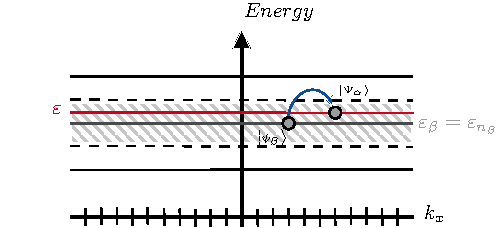
\includegraphics[scale=1.0]{figures/fig2.pdf}
  \caption{Scattering from $\ket{\psi_{\beta}(t,t')}$ to constant energy state $\ket{\Psi_{\alpha}(t,t')}$ due to scattering potential created by impurities.}
  \label{fig:2}
\end{figure}

\noindent
Here we need to undestand a state of this considering system only be represented by two independent quantum numbers which are $n$ energy eigen
states and $m$ quantum number which represents the qunatized momentum in $x$ direction values. Lets calculate the scattering amplitutde of the above mentioned scattering scenario using the equation derived in \eqref{4.18}.
\begin{equation} \label{4.21}
  \begin{aligned}
    a_{\alpha\beta}(\mb{k'},\mb{k},t,t') & =
    -
    \frac{i}{\hbar}
    \int_{0}^t dt_1 \;
    \bra{\psi_{\beta,\mb{k'}}(t_1,t')}
    V(\mb{r}) \ket{\psi_{\alpha,\mb{k}}(t_1,t')} \\
    & =
    -
    \frac{i}{\hbar}
    \int_{0}^t dt_1 \;
    e^{\frac{i}{\hbar}\qty(\varepsilon_{\beta} - \varepsilon)t_1}
    \bra{\phi_{\beta,\mb{k'}}(t')}
    V(\mb{r}) \ket{\phi_{\alpha,\mb{k}}(t')}
  \end{aligned}
\end{equation}
Next assuimg this scenario for long time $t \rightarrow \infty$ we can turn this integral into a delta distrubution as follows
\begin{equation} \label{4.22}
  \begin{aligned}
    a_{\alpha\beta}(\mb{k'},\mb{k},t,t') & =
    -
    \frac{i}{\hbar}
    \lim_{t \rightarrow \infty}\qty[
      \int_{-t/2}^{t/2} dt_1 \;
      e^{\frac{i}{\hbar}\qty(\varepsilon_{\beta} - \varepsilon)t_1}
      \bra{\phi_{\beta,\mb{k'}}(t')}
      V(\mb{r}) \ket{\phi_{\alpha,\mb{k}}(t')}
    ] \\
    & =
    -2\pi i \delta(\varepsilon_{\beta} - \varepsilon)
    \bra{\phi_{\beta,\mb{k'}}(t')}
    V(\mb{r}) \ket{\phi_{\alpha,\mb{k}}(t')}
  \end{aligned}
\end{equation}

\noindent
Now lets consider about the inner product of the above derivation. Using completeness properties we can write that as follows
\begin{equation} \label{4.23}
  \begin{aligned}
    Q & \equiv
    \bra{\phi_{\beta,\mb{k'}}(t')}
    V(\mb{r}) \ket{\phi_{\alpha,\mb{k}}(t')} \\
    & =
    \sum_{\mb{k}}\sum_{\mb{k'}}
    \braket{\phi_{\beta,\mb{k'}}(t')}{\mb{k'}}
    \mel{\mb{k'}}{V(\mb{r})}{\mb{k}}
    \braket{\mb{k}}{\phi_{\alpha,\mb{k}}(t')}
  \end{aligned}
\end{equation}
and seperating $x$ and $y$ directional momentums we can modify this as follows (Assuming $L_y \rightarrow \infty$) and since we assumed that $L_y \rightarrow \infty$
\begin{equation} \label{4.24}
  \begin{aligned}
    Q & \equiv
    \bra{\phi_{\beta,\mb{k'}}(t')}
    V(\mb{r}) \ket{\phi_{\alpha,\mb{k}}(t')} \\
    & =
    \sum_{k_x}\sum_{{k'}_x}
    \int_{-\infty}^{\infty} \int_{-\infty}^{\infty} dk_y d{k'}_y \;
    \phi_{\beta}(\mb{k'},t')
    \mel{\mb{k'}}{V(\mb{r})}{\mb{k}}
    \phi_{\alpha}(\mb{k},t').
  \end{aligned}
\end{equation}
For a random white scattering potential we can represent the inner product of scattering potential with momentum as a constant value as
\begin{equation} \label{4.25}
  V_{\mb{k'},\mb{k}} \equiv \mel{\mb{k'}}{V(\mb{r})}{\mb{k}}.
\end{equation}

\noindent
In this study, the perturbation potential is assumed to be formed by an ensemble of randomly distributed impurities, since randomimpurities iin a disorded metal is a better approximation for experimental results.

\noindent
Consider $N_{imp}$ identical impurities positioned at the randomly distributed but fixed potions $\mb{r}_i$. The elastic scattering potential $V(\mb{r})$ is then given by the sum over uncorrelated single impurity potentials $\upsilon(\mb{r})$
\begin{equation} \label{4.26}
  V(\mb{r}) \equiv
  \sum_{i=1}^{N_{imp}}
  \upsilon (\mb{r}-\mb{r}_i).
\end{equation}
Now assume that the perturbation $V(\mb{r})$ is a Gaussian random potential where one can choose the zero of enerrgy such that the potential is zero on average. This model characterized by [*Ref: e.Akkermans G. Montambaux]
\begin{equation} \label{4.27}
  \expval{\upsilon(\mb{r})}_{imp} =0
\end{equation}
\begin{equation} \label{4.28}
  \expval{\upsilon(\mb{r})\upsilon(\mb{r'})}_{imp} = \Upsilon(\mb{r}-\mb{r'})
\end{equation}
where $\expval{\cdot}_{imp}$ denoted the average over realizations of the impurity disorder. In addition, this model assume that $\upsilon (\mb{r}-\mb{r'})$ only dependes on the position difference $|\mb{r}-\mb{r'}|$ and it decays with a characteristic leangth $r_c$. Since the study considers the case where the waveleagth of radiation or scattering electrons is much faster than $r_c$, it is good approximation to make two-point correlation function to be
\begin{equation} \label{4.29}
  \expval{\upsilon(\mb{r})\upsilon(\mb{r'})}_{imp} = \Upsilon_{imp}^2\delta(\mb{r}-\mb{r'})
\end{equation}
and a random potential $V(\mb{r})$ with this property is called white noise [*Ref: e.Akkermans G. Montambaux]. Then we can choose approximately total scattering potential as
\begin{equation} \label{4.30}
  V(\mb{r}) =
  \sum_{i=1}^{N_{imp}}
  \Upsilon_{imp} \delta(\mb{r}-\mb{r}_i).
\end{equation}

\noindent
Since $\braket{\mb{r}}{\mb{k}} = \frac{1}{\sqrt{L_xL_y}} \exp(-i[k_xx + k_yy]),$ we can calculate the Eq. \eqref{4.25} using this assumption as follows
\begin{equation} \label{4.31}
  \begin{aligned}
    V_{\mb{k'},\mb{k}}
    & = \mel{\mb{k'}}{V(\mb{r})}{\mb{k}} \\
    & = \mel**{\mb{k'}}{\sum_{i=1}^{N_{imp}}
    \Upsilon_{imp} \delta(\mb{r}-\mb{r}_i)}{\mb{k}} \\
    & = \mel**{\mb{k'}}{\sum_{i=1}^{N_{imp}}
    \Upsilon_{imp} \delta(x-x_i)\delta(y-y_i)}{\mb{k}} \\
    & =
    \sum_{i=1}^{N_{imp}}
    \int_{-\infty}^{\infty} dy\;
    \frac{1}{\sqrt{L_xL_y}} e^{ik'_y y} \delta(y-y_i) \frac{1}{\sqrt{L_xL_y}} e^{-i{k}_y y}
    \mel**{k'_x}{\Upsilon_{imp} \delta(x-x_i)}{k_x} \\
    &=
    \sum_{i=1}^{N_{imp}} \frac{1}{{L_xL_y}}
    e^{i(k'_y - k_y )y}
    \mel**{k'_x}{\Upsilon_{imp} \delta(x-x_i)}{k_x}
  \end{aligned}
\end{equation}
Assuming the total  umber of scatterers $N_{imp}$ is macroscopically large and for each impurity will produce same impurity potential($V_{k'_x,k_x}$) (\textcolor{red}{this is not sure and we need to prove this somehonw or we need to bring the $V_{\mb{k},\mb{k'}}$ without calculations})for every $x$-directional momentum pairs, we can achieve following expression
\begin{equation} \label{4.32}
  \begin{aligned}
    V_{\mb{k'},\mb{k}}
    & =
    V_{k'_x,k_x}
    \frac{N_{imp}}{L_y L_x} \int_{-\infty}^{\infty} dy_i\;
    e^{i\qty({k'}_y - k_y)y_i} \\
    & =
    \eta_{imp} V_{k'_x,k_x} \delta(k'_y - k_y)
  \end{aligned}
\end{equation}
where
\begin{equation} \label{4.33}
  V_{{k'}_x,k_x} \equiv
  \mel**{k'_x}{\Upsilon_{imp} \delta(x-x_i)}{k_x}
\end{equation}
is constant value for every $i$ impurity and $\eta_{imp}$ is number of impurities in a unit area. It is important to notice that $\ket{k_x} = e^{-ik_xx}$.\\

\noindent
Therefore, using the Eq. \eqref{3.36}, the Eq. \eqref{4.24} modified to (we can change varable $t' \rightarrow t$)
\begin{equation} \label{4.34}
  \begin{aligned}
    Q & =
    \sum_{k_x}\sum_{{k'}_x}
    {\eta_{imp} V_{{k'}_x,k_x}}
    \int_{-\infty}^{\infty} \int_{-\infty}^{\infty} dk_y d{k'}_y \;
    \delta({k'}_y - k_y)
    \\
    & \times
    \sqrt{L_x}
    \exp(
      -ib\sin(2\omega t)
    )
    \exp(
      i{k'}_y  \qty[d\sin(\omega t) + {y'}_0]
    )
    \tilde{\chi}_{n_{\beta}}\qty({k'}_y -g\cos(\omega t))
    \\
    & \times
    \sqrt{L_x}
    \exp(
      ib\sin(2\omega t)
    )
    \exp(
      -ik_y  \qty[d\sin(\omega t) + y_0]
    )
    \tilde{\chi}_{n_{\alpha}}\qty(k_y -g\cos(\omega t))
  \end{aligned}
\end{equation}
and we can simplify this as
\begin{equation} \label{4.35}
  \begin{aligned}
    Q =
    \sum_{k_x}\sum_{{k'}_x} &
    {\eta_{imp} L_x V_{{k'}_x,k_x}}
    \int_{-\infty}^{\infty} dk_y \;
    \\
    & \times
    \exp(
      i{k}_y {y'}_0
    )
    \tilde{\chi}_{n_{\beta}}\qty({k}_y -g\cos(\omega t))
    \exp(
      -ik_y y_0
    )
    \tilde{\chi}_{n_{\alpha}}\qty(k_y -g\cos(\omega t))
  \end{aligned}
\end{equation}
and this can re-write as
\begin{equation} \label{4.36}
  \begin{aligned}
    Q =
    \sum_{k_x}\sum_{{k'}_x}
    {\eta_{imp} L_x V_{{k'}_x,k_x}} I
  \end{aligned}
\end{equation}
where
\begin{equation} \label{4.37}
  \begin{aligned}
    I \equiv
    \int_{-\infty}^{\infty} dk_y \;
    \tilde{\chi}_{n_{\beta}}\qty(k_y -g\cos(\omega t))
    \tilde{\chi}_{n_{\alpha}}\qty(k_y -g\cos(\omega t))
    \exp(
      -ik_y  \qty[y_0 - {y'}_0  ]
    ).
  \end{aligned}
\end{equation}

\noindent
To avoid the energy tramision from external high-frequency field and electrons in the system, the applied radiation should be purely dressing field. Therefore, the only effect of the dressing field on 2DEG is the renormalization of the probability of elastic electron scattering within same Landau level $(n_{\alpha} = n_{\beta})$. Therefore Eq. \eqref{4.37} can be modified to
\begin{equation} \label{4.38}
  \begin{aligned}
    I \equiv
    \int_{-\infty}^{\infty} dk_y \;
    \tilde{\chi}_{n_{\beta}}^2 \qty(k_y -g\cos(\omega t))
    \exp(
      -ik_y  \qty[y_0 - {y'}_0  ]
    ).
  \end{aligned}
\end{equation}

\noindent
Lets consider about this integral and we can calculate it as using the following subtitution. Let
\begin{equation} \label{4.39}
  {k}_y -g\cos(\omega t) = \bar{k}_y \longrightarrow d{k}_y = d\bar{k}_y
\end{equation}
and this leads to
\begin{equation} \label{4.40}
    I \equiv
    2\pi \times \frac{1}{2\pi}
    \int_{-\infty}^{\infty} d\bar{k}_y \;
    \tilde{\chi}_{n_{\alpha}}^2 \qty(\bar{k}_y)
    \exp(
      -i\qty(\bar{k}_y + g\cos(\omega t)) \qty(y_0 - {y'}_0)
    ).
\end{equation}
Using Fourier transform of Gauss-Hermite functions and convolution theorem we can write this as
\begin{equation} \label{4.41}
    I \equiv
    {2\pi}
    \exp(g[{y'}_0 - y_0]\cos(\omega t))
    \int_{-\infty}^{\infty} dy \;
    {\chi}_{n_{\beta}}\qty(y)
    {\chi}_{n_{\beta}}\qty(y_0 - {y'}_0 - y).
\end{equation}
Therefore the scatterng amplitude \eqref{4.22} will modified to
\begin{equation} \label{4.42}
  \begin{aligned}
    a_{\alpha\beta}({k'}_x,k_x,t)  =
    -2\pi i
    \delta(\varepsilon_{\beta} - \varepsilon)
    \sum_{k_x}\sum_{{k'}_x}
    {\eta_{imp} L_x V_{{k'}_x,k_x}} I
  \end{aligned}
\end{equation}
Consideirng qunatized momentum given in $x$ direction derived in Eq. \eqref{1.53}, we can identify the non-zero values for scattering amplitude using following conditions
\begin{equation} \label{4.43}
    {k'}_x = \frac{p_{x_{\beta}}}{\hbar} = m' \frac{2\pi}{L_x}
    \quad \text{and} \quad
    k_x = \frac{p_{x_{\alpha}}}{\hbar} = m \frac{2\pi}{L_x}.
\end{equation}
Then we can simplfied scattering amplitude for given ${k'}_x$ and $k_x$ as
\begin{equation} \label{4.44}
  \begin{aligned}
    a_{\alpha\beta}({k'}_x,k_x,t)  =
    -2\pi i
    \delta(\varepsilon_{\beta} - \varepsilon)
    \eta_{imp} L_x V_{{k'}_x,k_x}&
    \exp(g[{y'}_0 - y_0]\cos(\omega t)) \\
    & \times
    \int_{-\infty}^{\infty} dy \;
    {\chi}_{n_{\beta}}\qty(y)
    {\chi}_{n_{\beta}}\qty(y_0 - {y'}_0 - y)
  \end{aligned}
\end{equation}
Since this scattering amplitude is time-periodic we can write this as a Fourier series expansion
\begin{equation} \label{4.45}
    a_{\alpha\beta}({k'}_x,k_x,t) =
    \sum_{l=-\infty}^{\infty} a^l_{\alpha\beta}({k'}_x,k_x) e^{-il\omega t}.
\end{equation}
In addition, using Jacobi-Anger expansion
\begin{equation} \label{4.46}
    e^{iz\cos(\theta)} = \sum_{l=-\infty}^{\infty} i^l J_l\qty(z) e^{-il\theta}
\end{equation}
we can re-write the Eq.\eqref{4.44} as folllows
\begin{equation} \label{4.47}
  \begin{aligned}
    a_{\alpha\beta}({k'}_x,k_x,t)  =
    -2\pi i
    \delta(\varepsilon_{\beta} - \varepsilon)
    \eta_{imp} L_x V_{{k'}_x,k_x}&
    \sum_{l=-\infty}^{\infty} i^l J_l\qty(g[{y'}_0 - y_0]) e^{-il\omega t}\\
    & \times
    \int_{-\infty}^{\infty} dy \;
    {\chi}_{n_{\beta}}\qty(y)
    {\chi}_{n_{\beta}}\qty(y_0 - {y'}_0 - y)
  \end{aligned}
\end{equation}
\begin{equation} \label{4.48}
  \begin{aligned}
    a_{\alpha\beta}({k'}_x,k_x,t)  =
    \sum_{l=-\infty}^{\infty}
    -2\pi i^{l+1} &
    \delta(\varepsilon_{\beta} - \varepsilon)
    \eta_{imp} L_x V_{{k'}_x,k_x}
    J_l\qty(g[{y'}_0 - y_0]) \\
    & \times
    \int_{-\infty}^{\infty} dy \;
    {\chi}_{n_{\beta}}\qty(y)
    {\chi}_{n_{\beta}}\qty(y_0 - {y'}_0 - y) e^{-il\omega t}
  \end{aligned}
\end{equation}
Then we can identified the Fourier series component as
\begin{equation} \label{4.49}
    a^l_{\alpha\beta}({k'}_x,k_x) =
    -2\pi i^{l+1}
    \delta(\varepsilon_{\beta} - \varepsilon)
    \eta_{imp} L_x V_{{k'}_x,k_x}
    J_l\qty(g[{y'}_0 - y_0])
    \int_{-\infty}^{\infty} dy \;
    {\chi}_{n_{\beta}}\qty(y)
    {\chi}_{n_{\beta}}\qty(y_0 - {y'}_0 - y)
\end{equation}
Now one can introduce the definition of the \textit{transition probability matrix} as
\begin{equation} \label{4.50}
    \qty(A_{\alpha\beta}({k'}_x,k_x))_{l,l'} \equiv
    a^l_{\alpha\beta}({k'}_x,k_x)\qty[a^{l'}_{\alpha\beta}({k'}_x,k_x)]^{*}
\end{equation}
and this becomes
\begin{equation} \label{4.51}
  \begin{aligned}
      \qty(A_{\alpha\beta}({k'}_x,k_x))_{l,l'} & =
      \qty[{ 2 \pi \eta_{imp} L_x |V_{{k'}_x,k_x}|}]^2
      J_l\qty(g[{y'}_0 - y_0]) J_{l'}\qty(g[{y'}_0 - y_0])
      \delta^2(\varepsilon_{\beta} - \varepsilon) \\
      & \times
      \int_{-\infty}^{\infty} dy \;
      {\chi}_{n_{\beta}}\qty(y)
      {\chi}_{n_{\beta}}\qty(y_0 - {y'}_0 - y)
      \int_{-\infty}^{\infty} d\bar{y} \;
      {\chi}_{n_{\beta}}\qty(\bar{y})
      {\chi}_{n_{\beta}}\qty(y_0 - {y'}_0 - \bar{y}).
  \end{aligned}
\end{equation}

\noindent
We can reduce these intragal into one variable and derive
\begin{equation} \label{4.52}
  \begin{aligned}
      \qty(A_{\alpha\beta}({k'}_x,k_x))_{l,l'} =
      \qty[{ 2 \pi \eta_{imp} L_x |V_{{k'}_x,k_x}|}]^2 &
      J_l\qty(g[{y'}_0 - y_0]) J_{l'}\qty(g[{y'}_0 - y_0])
      \delta^2(\varepsilon_{\beta} - \varepsilon) \\
      & \times
      \qty|
      \int_{-\infty}^{\infty} dy \;
      {\chi}_{n_{\beta}}\qty(y)
      {\chi}_{n_{\beta}}\qty(y_0 - {y'}_0 - y)|^2.
  \end{aligned}
\end{equation}
Then desribing the square of the delta distribution using following procedure
\begin{equation} \label{4.53}
    \delta^2(\varepsilon) =
    \delta(\varepsilon)\delta(0) =
    \frac{\delta(\varepsilon)}{2\pi \hbar}
    \int_{-t/2}^{t/2} e^{i0\times t'/\hbar} dt'\; =
    \frac{\delta(\varepsilon)t}{2\pi \hbar}
\end{equation}
one can modify our derivation in Eq. \eqref{4.51} as
\begin{equation} \label{4.54}
  \begin{aligned}
      \qty(A_{\alpha\beta}({k'}_x,k_x))_{l,l'} =
      \qty[{ 2 \pi \eta_{imp} L_x |V_{{k'}_x,k_x}|}]^2 &
      J_l\qty(g[{y'}_0 - y_0]) J_{l'}\qty(g[{y'}_0 - y_0])
      \delta(\varepsilon_{\beta} - \varepsilon)
      \frac{t}{2\pi \hbar}\\
      & \times
      \qty|
      \int_{-\infty}^{\infty} dy \;
      {\chi}_{n_{\beta}}\qty(y)
      {\chi}_{n_{\beta}}\qty(y_0 - {y'}_0 - y)|^2.
  \end{aligned}
\end{equation}
Then performing thetime derivation of each matrix element yeild the \textit{transition amplitude matrix} as folllows
\begin{equation} \label{4.55}
  \begin{aligned}
    \Gamma_{\alpha\beta}^{ll'}({k'}_x,k_x) &  \equiv
    \frac{d \qty(A_{\alpha\beta}({k'}_x,k_x))_{l,l'}}{dt} \\
    & =
    \Lambda |V_{{k'}_x,k_x}|^2
    \delta(\varepsilon_{\beta} - \varepsilon)
    J_l\qty(g[{y'}_0 - y_0]) J_{l'}\qty(g[{y'}_0 - y_0])
    \qty|
    \int_{-\infty}^{\infty} dy \;
    {\chi}_{n_{\beta}}\qty(y)
    {\chi}_{n_{\beta}}\qty(y_0 - {y'}_0 - y)|^2
  \end{aligned}
\end{equation}
where
\begin{equation} \label{4.56}
    \Lambda \equiv
    \frac { 2\pi \eta_{imp}^2 L_x^2}{ \hbar}
\end{equation}

\noindent
Now using defintion of $y_0$ given in Eq. \eqref{1.11} we can write that
\begin{equation} \label{4.57}
    y_0 - {y'}_0 =
    - \frac{p_{x_{\alpha}}}{eB} + \frac{p_{x_{\beta}}}{eB} =
    \frac{\hbar {k'}_x}{eB} - \frac{\hbar {k}_x}{eB} =
    \frac{\hbar}{eB} \qty[{k'}_x - {k}_x]
\end{equation}
and this leads Eq. \eqref{4.56} to
\begin{equation} \label{4.58}
  \begin{aligned}
    \Gamma_{\alpha\beta}^{ll'}({k'}_x,k_x) =
    \Lambda |V_{{k'}_x,k_x}|^2
    \delta(\varepsilon_{\beta} - \varepsilon) &
    J_l\qty(\frac{g\hbar}{eB}[{k}_x - {k'}_x])
    J_{l'}\qty(\frac{g\hbar}{eB}[{k}_x - {k'}_x]) \\
    & \times
    \qty|
    \int_{-\infty}^{\infty} dy \;
    {\chi}_{n_{\beta}}\qty(y)
    {\chi}_{n_{\beta}}\qty(\frac{\hbar}{eB} \qty[{k'}_x - {k}_x] - y)|^2
  \end{aligned}
\end{equation}

\noindent
An impurity average of white noise potential allows to identify $\expval{|V_{{k'}_x,k_x}|^2} = V_{imp}$ and the inverse scattering time matrix is the sum over all momentum over the transition probability matrix
\begin{equation} \label{4.59}
    \qty(\frac{1}{\tau(\varepsilon,k_x)})^{ll'}_{\alpha\beta} \equiv
    \frac{1}{L_x} \sum_{{k'}_x}
    \expval**{\Gamma_{\alpha\beta}^{ll'}({k'}_x,k_x)}_{imp}
\end{equation}
and this implies
\begin{equation} \label{4.60}
  \begin{aligned}
    \Gamma_{\alpha\beta}^{ll'}({k'}_x,k_x) =
    \frac{\Lambda V_{imp}}{L_x} \sum_{{k'}_x}
    \delta(\varepsilon_{\beta} - \varepsilon) &
    J_l\qty(\frac{g\hbar}{eB}[{k}_x - {k'}_x])
    J_{l'}\qty(\frac{g\hbar}{eB}[{k}_x - {k'}_x]) \\
    & \times
    \qty|
    \int_{-\infty}^{\infty} dy \;
    {\chi}_{n_{\beta}}\qty(y)
    {\chi}_{n_{\beta}}\qty(\frac{\hbar}{eB} \qty[{k'}_x - {k}_x] - y)|^2
  \end{aligned}
\end{equation}
For the 1-dimentional case introduce the momentum continuum limit as folllows
\begin{equation} \label{4.61}
    \frac{1}{L_x} \sum_{{k'}_x} \longrightarrow
    \frac{1}{2\pi}\int d {k'}_x
\end{equation}
and this leads to
\begin{equation} \label{4.62}
  \begin{aligned}
    \qty(\frac{1}{\tau(\varepsilon,k_x)})^{ll'}_{\alpha\beta} =
    \frac{\Lambda V_{imp}}{2\pi}
    \delta(\varepsilon_{\beta} - \varepsilon)
    \int_{-\infty}^{\infty} d {k'}_x
    &
    J_l\qty(\frac{g\hbar}{eB}[{k}_x - {k'}_x])
    J_{l'}\qty(\frac{g\hbar}{eB}[{k}_x - {k'}_x]) \\
    & \times
    \qty|
    \int_{-\infty}^{\infty} dy \;
    {\chi}_{n_{\beta}}\qty(y)
    {\chi}_{n_{\beta}}\qty(\frac{\hbar}{eB} \qty[{k'}_x - {k}_x] - y)|^2
  \end{aligned}
\end{equation}
Using following subtitution
\begin{equation} \label{4.63}
    y = \frac{\hbar \bar{k}}{eB} \longrightarrow
    dy = \frac{\hbar }{eB} d\bar{k}
\end{equation}
we can modify above derivation as
\begin{equation} \label{4.64}
  \begin{aligned}
    \qty(\frac{1}{\tau(\varepsilon,k_x)})^{ll'}_{\alpha\beta} =
    \frac{\Lambda V_{imp}}{2\pi}
    \delta(\varepsilon_{\beta} - \varepsilon)
    \int_{-\infty}^{\infty} d {k'}_x
    &
    J_l\qty(\frac{g\hbar}{eB}[{k}_x - {k'}_x])
    J_{l'}\qty(\frac{g\hbar}{eB}[{k}_x - {k'}_x]) \\
    & \times
    \qty(\frac{\hbar }{eB})^2
    \qty|
    \int_{-\infty}^{\infty} d\bar{k} \;
    {\chi}_{n_{\beta}}\qty(\frac{\hbar}{eB}\bar{k})
    {\chi}_{n_{\beta}}\qty(\frac{\hbar}{eB} \qty[{k'}_x - {k}_x - \bar{k}])|^2,
  \end{aligned}
\end{equation}
% Since squared Guess-Hermite functions are even function around zero we can re-write above derived expression as
% \begin{equation} \label{4.65}
%   \begin{aligned}
%     \qty(\frac{1}{\tau(\varepsilon,k_x)})^{ll'}_{\alpha\beta} =
%     \frac{\Lambda V_{imp}}{2\pi}
%     \delta(\varepsilon_{\beta} - \varepsilon)
%     \int_{-\infty}^{\infty} d {k'}_x
%     &
%     J_l\qty(\frac{g\hbar}{eB}[{k}_x - {k'}_x])
%     J_{l'}\qty(\frac{g\hbar}{eB}[{k}_x - {k'}_x]) \\
%     & \times
%     \frac{\hbar }{eB}
%     \int_{-\infty}^{\infty} d\bar{k} \;
%     \tilde{\chi}^2_{n_{\beta}}\qty(\frac{\hbar}{eB}\bar{k})
%     \tilde{\chi}^2_{n_{\beta}}\qty(\frac{\hbar}{eB}
%     \qty[\bar{k} - ({k}_x  - {k'}_x)])
%   \end{aligned}
% \end{equation}
and finally we can derive our expression for the \textit{inverse
scattering time matrix} for $N$th Landau level (let $n_{\alpha} = n_{\beta} = N$)
\begin{equation} \label{4.65}
  \begin{aligned}
    \qty(\frac{1}{\tau(\varepsilon,k_x)})^{ll'}_{N} =
    \frac { \eta_{imp}^2 L_x^2 \hbar V_{imp}}{\qty(eB)^2}
    \delta(\varepsilon - \varepsilon_{N})
    \int_{-\infty}^{\infty} d {k'}_x
    &
    J_l\qty(\frac{g\hbar}{eB}[{k}_x - {k'}_x])
    J_{l'}\qty(\frac{g\hbar}{eB}[{k}_x - {k'}_x]) \\
    & \times
    \qty|
    \int_{-\infty}^{\infty} d\bar{k} \;
    {\chi}_{N}\qty(\frac{\hbar}{eB}\bar{k})
    {\chi}_{N}\qty(\frac{\hbar}{eB} \qty[{k'}_x - {k}_x - \bar{k}])|^2.
  \end{aligned}
\end{equation}
\hfill$\blacksquare$
